\documentclass[11pt]{article}
\usepackage{amsmath, amssymb}
\usepackage{geometry}
\geometry{margin=1in}
\usepackage{fancyhdr}
\usepackage{lastpage}
\usepackage{parskip} % Better paragraph spacing
\usepackage{titlesec} % Better section formatting
\usepackage{graphicx}
\usepackage{float}
\usepackage[most]{tcolorbox}
\usepackage{lmodern}
\usepackage{caption}
\usepackage{hyperref}
\usepackage{listings}
\usepackage{xcolor}

\definecolor{codegreen}{rgb}{0,0.6,0}
\definecolor{codegray}{rgb}{0.5,0.5,0.5}
\definecolor{codepurple}{rgb}{0.58,0,0.82}
\definecolor{backcolour}{rgb}{0.95,0.95,0.92}

% Define code styling
\lstdefinestyle{mystyle}{
    backgroundcolor=\color{backcolour},
    commentstyle=\color{codegreen},
    keywordstyle=\color{magenta},
    numberstyle=\tiny\color{codegray},
    stringstyle=\color{codepurple},
    basicstyle=\ttfamily\footnotesize,
    breakatwhitespace=false,
    breaklines=true,
    captionpos=b,
    keepspaces=true,
    numbers=left,
    numbersep=5pt,
    showspaces=false,
    showstringspaces=false,
    showtabs=false,
    tabsize=2
}

\lstset{style=mystyle}

% Define commands for reusable content
\newcommand{\coursename}{COM-402 Information Security and Privacy}
\newcommand{\lecturenum}{08}
\newcommand{\lecturedate}{10/11/2025}
\newcommand{\professor}{Mathias Payer}

\hypersetup{colorlinks=true,linkcolor=blue,urlcolor=blue}

% Configure section spacing
\titlespacing*{\section}{0pt}{2ex plus 1ex minus .2ex}{1.5ex plus .2ex}
\titlespacing*{\subsection}{0pt}{1.5ex plus 1ex minus .2ex}{1ex plus .2ex}
% Header / Footer
\pagestyle{fancy}
\fancyhf{}
\fancyhead[L]{\coursename}
\fancyhead[R]{Lecture \lecturenum}
\fancyfoot[L]{EPFL - Computer Science}
\fancyfoot[C]{Author: Jonathan Dutoit}
\fancyfoot[R]{Page \thepage\ of \pageref{LastPage}}

\begin{document}

\begin{center}
  {\large EPFL - Computer Science} \\[0.5em]
  {\Large \textbf{\coursename}} \\[0.5em]
  {\large Lecture \lecturenum\ --- \lecturedate} \\[0.5em]
  {\large Author: Jonathan Dutoit} \\[0.5em]
  {\large Professor: \professor} \\[0.5em]
\end{center}

\vspace{1cm}
\begin{center}
  {\LARGE \textbf{Mobile Security}}
\end{center}
\vspace{1cm}

\section*{Learning goals}

\begin{itemize}
	\item Differentiate the security goals of mobile systems from desktop/server systems
	\item Awareness of security trade-offs for Android (vs. iOS)
	\item Understand security mitigations deployed by vendors
\end{itemize}

\vspace{0.5cm}

\begin{center}
  {\LARGE \textbf{Mobile Security Motivation}}
\end{center}
\vspace{0.5cm}
\textbf{Computing Revolutions}

1. Data processing (in the 70ies) \\
2. Personal Computing (in the 80ies) \\
3. Internet (in the 90ies): \textcolor{orange}{Computers now exposed to everyone else}\\ 
4. Mobile Computing (in the 00's): \textcolor{orange}{Mobile ecosystem keeps personal data}\\
5. Social (in the 10's): \textcolor{orange}{Nightmare for privacy/personal data} \\
6. AI? (20's): \textcolor{orange}{The web is dead: everything is in silos}

\textbf{Why is mobile security hard?} On a phone, a bunch of software is running from multiple sources...

% Quick centered image
\begin{figure}[H]
    \centering
    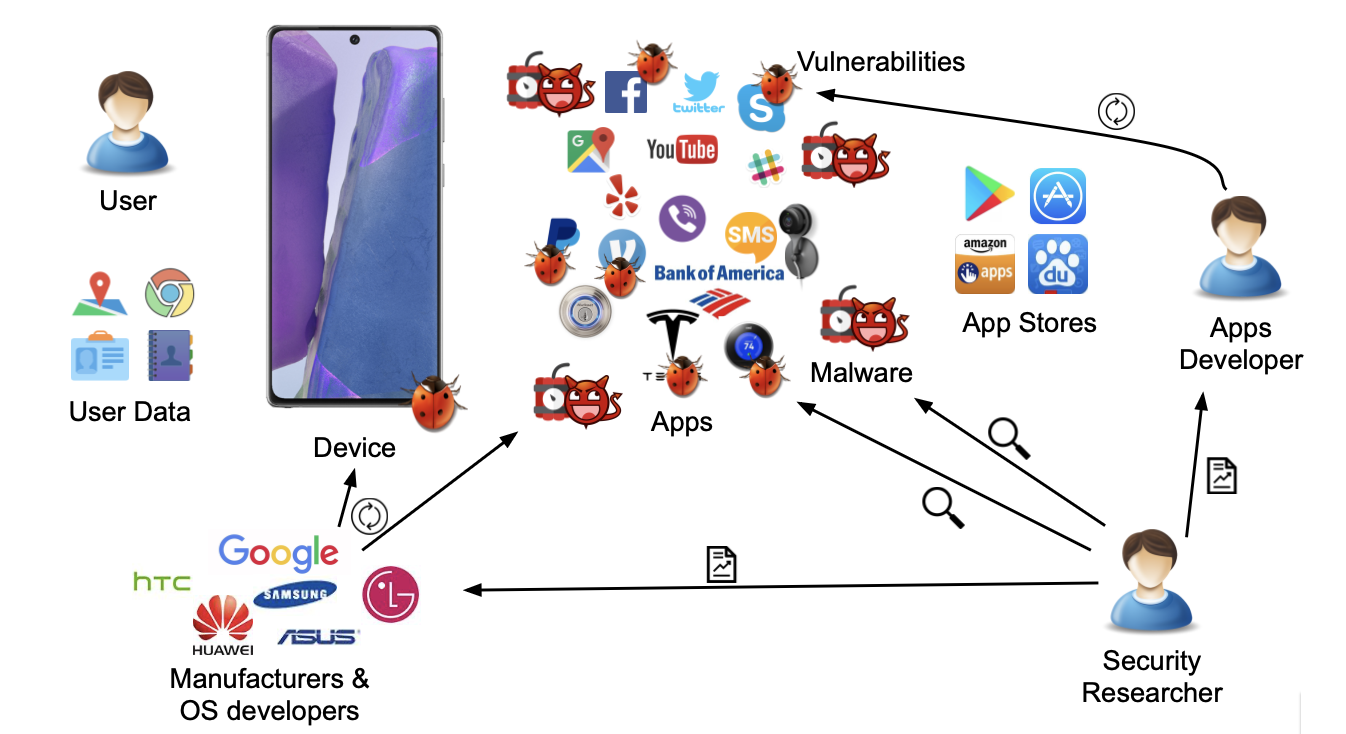
\includegraphics[width=0.7\textwidth]{mobile-system}
    \label{fig:LABEL}
\end{figure}

\section*{Types of Malware: Repackaging / Look-alike Malware}

Download app from app market (e.g., Google Play Store)

Unpack and reverse engineer app $\Rightarrow$ This is relatively easy on Android

Modify and add code
\begin{itemize}
	\item Add ads
	\item Require more permissions than original app to steal user data
	\item Escalate privileges using exploits to deploy ransomware
	\item ...
\end{itemize}

Pack and publish modified version

\section*{Piracy of Digital Content}

Steal digital content from content providers. Platform needs support for secure audio and video playback. Premium content must not leave the decide!

Streaming services usually require platform with digital rights management (DRM) solutions to stream premium content (e.g., 4K streams)

You can't record your screen while watching Netflix nor directly read the video files. That's because Netflix software is managed by a different part of the phone called \textbf{Trusted Execution Environment}

DRM Solution: 
\begin{itemize}
	\item Google Widevine
	\item Microsoft PlayReady
\end{itemize}

\textbf{Broader: Political Instrument}

Takeaways: mobile security is very important and try to avoid making enemies with money. 

\vspace{0.5cm}

\begin{center}
  {\LARGE \textbf{Android Ecosystem and Security}}
\end{center}
\vspace{0.5cm}

\section*{Android Open Source Project (AOSP)}

Android is "\textbf{owned}" by Google. Code is made available through AOSP. 

Original Equipment Manufacturer (OEM) customizes code to their hardware. OEM adds proprietary components (e.g., for hardware support). For instance if you buy Xiaomi or Pixel phone, they look very different! 

Google Mobile Services (Google Play, YouTube, Google Maps, Gmail, ...) require OEM to comply with \underline{compatibility definition document}

\section*{From Chip to Android Phone}

% Quick centered image
\begin{figure}[H]
    \centering
    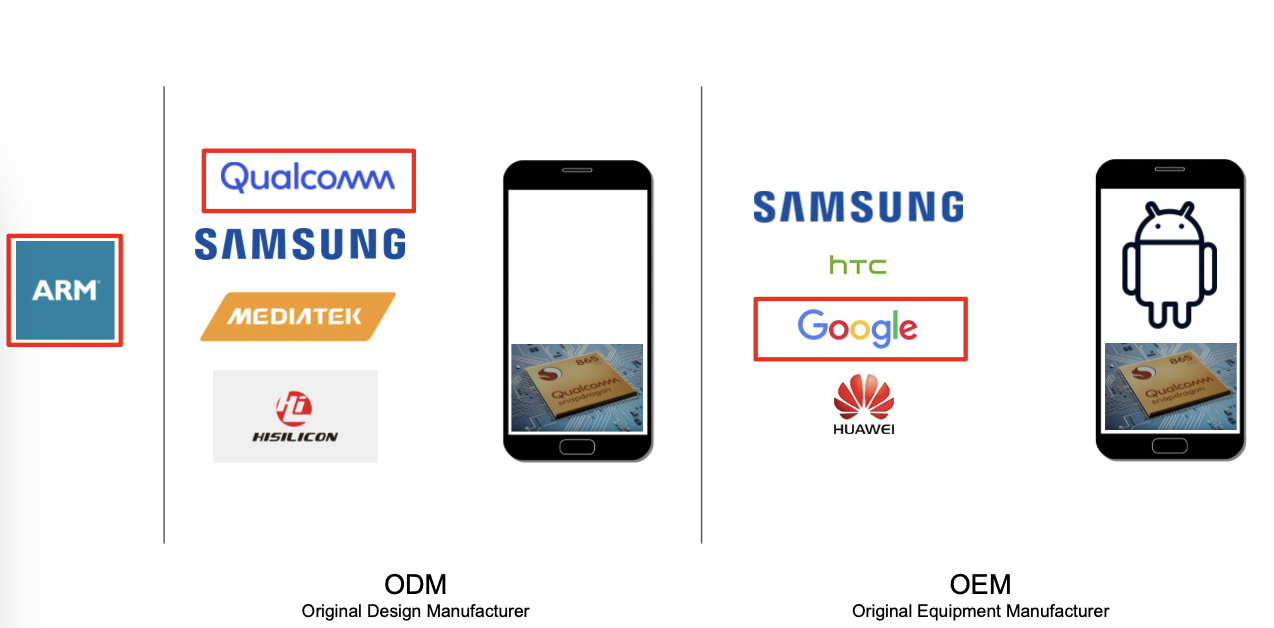
\includegraphics[width=0.8\textwidth]{chip}
    \label{fig:LABEL}
\end{figure}

\section*{The "Open" in AOSP}

Q: "How does setting a PIN/pattern/password work?"

1. Determine component that implements feature \\
2. Figure out AOSP release \\
3. Look for component in AOSP \\
4. Read code until you are satisfied \\

\section*{The "not-so-Open" in AOSP}

\begin{minipage}{0.6\textwidth}
Enrolling and verifying passwords is a security-sensitive feature \\

The backed of this feature is implemented by the Gatekeeper subsystem \\

This subsystem often uses the TEE and is usually platform-dependent ($\sim$ proprietary)
\begin{itemize}
	\item Guarantees stronger confidentiality
	\item Throttles consecutive failed attemps
\end{itemize}

\end{minipage}
\hfill
\begin{minipage}{0.4\textwidth}
\centering
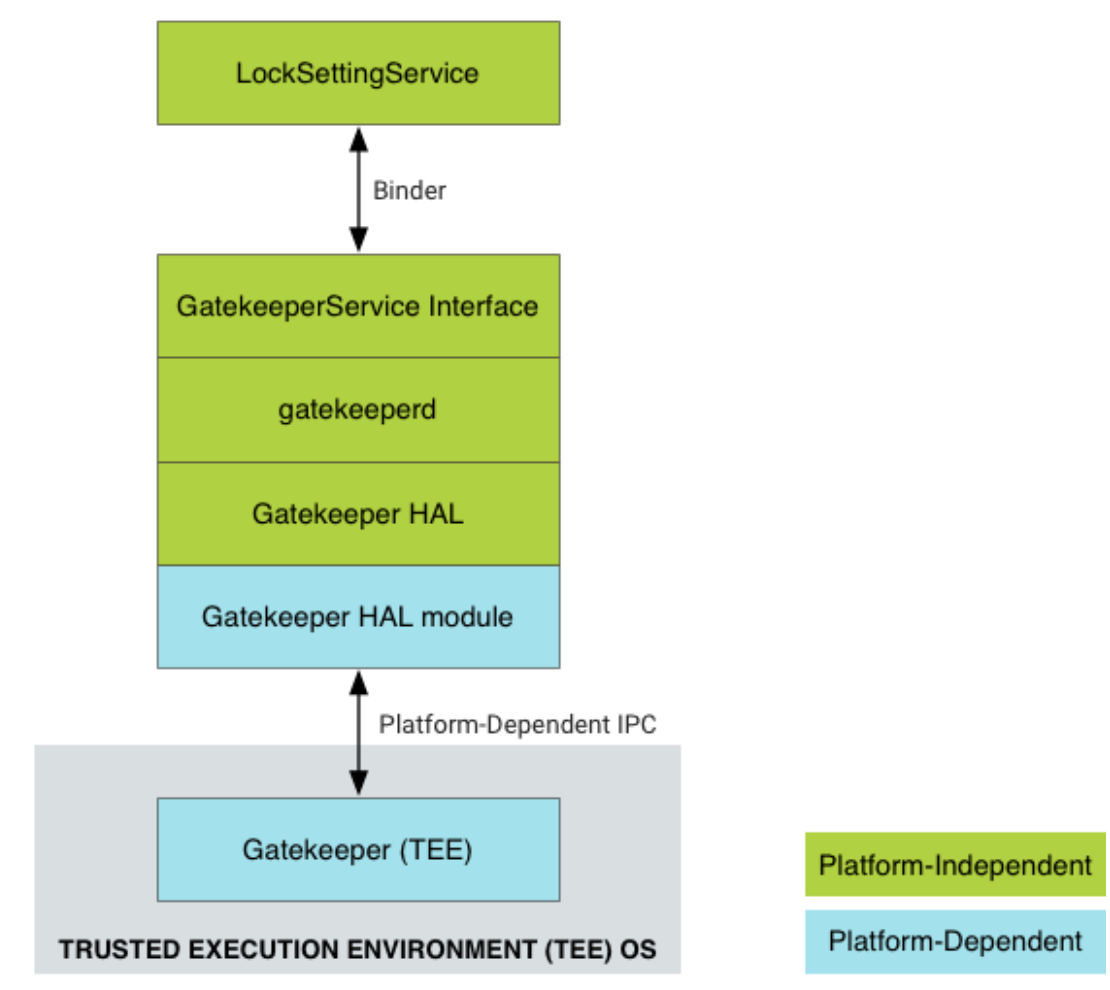
\includegraphics[width=\linewidth]{not-so-open}
\end{minipage}

\section*{Android Devices}

Many different players: Many different hardware manufacturers / OEMs who customize their software/hardware stack

Many different Android versions
\begin{itemize}
	\item Not all devices support all versions
	\item Some devices never get updates (tablets)
	\item Most devices get updates only for $\sim$ 3 years
	\item Android versions distribution secluded
\end{itemize}

\section*{What Android Version Would You Target?}

If you're building your own application, you must consider trade-offs between security and reachability 
% Quick centered image
\begin{figure}[H]
    \centering
    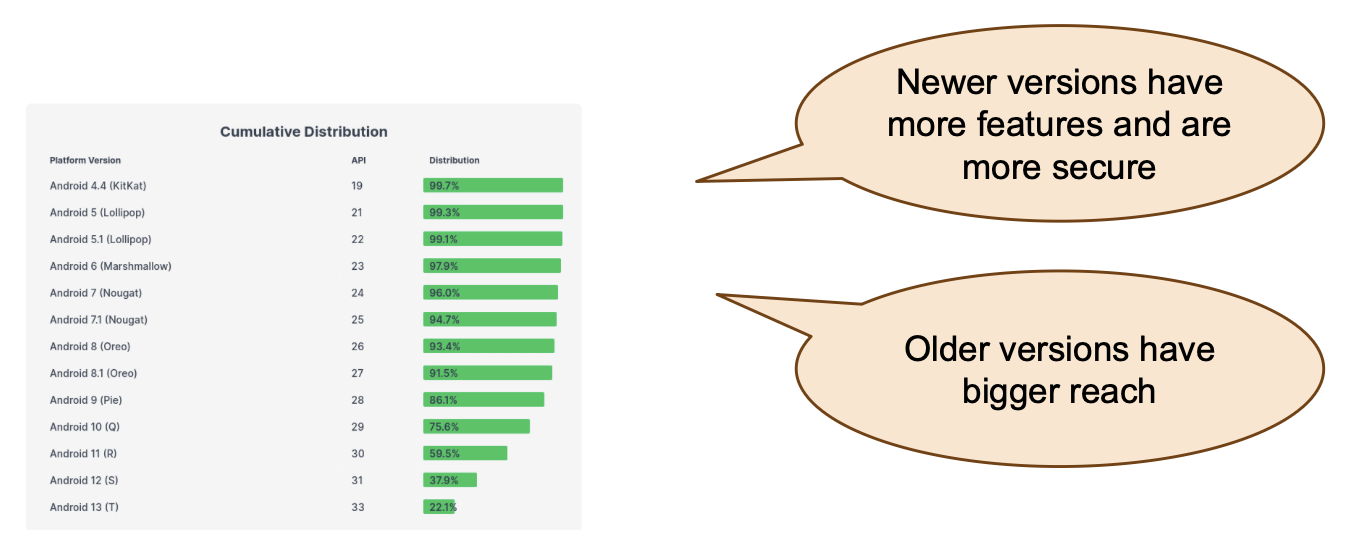
\includegraphics[width=1\textwidth]{version}
    \label{fig:LABEL}
\end{figure}

Android 10 devices still being sold (6 years old)

\section*{Android Fragmentation}

Fragmentation is the \textit{\textbf{biggest challenger}} for Android security

Thousands of devices with custom hardware and software

Customization makes development and patching tricky 

\section*{The Long Life of a Security Bug: Reporting}

1. Discovery: Security researchers (Google's or external) finds a bug \\
2. Disclosure: Report the bug to Google \\
3. Reception: 
\begin{itemize}
	\item $[$Hope the bug reaches the right Google employee$]$
	\item Google acknowledges the bug and will work on a fix
\end{itemize}

\newpage
\section*{The Long Life of a Security Bug: Fixing}
(Responsible) Coordinated Disclosure 

\begin{itemize}
	\item $[$ Wait n days, industry standard: 90 days $]$
	\item Publicly disclose bug
\end{itemize}

Security patch distribution
\begin{itemize}
	\item Google distributes the patches to other manufactures
	\item Patch is published as part of the \underline{Monthly Security Bulletin}
\end{itemize}

Supported Google devices get the patch. Vendors (e.g., Xiaomi) are advertised of found bugs. \textbf{Problem}: Vendors are always using a fork (own modifications) 

\section*{The perils of customization}

Google sends patch to third-party company X: Company X now needs to apply the patch to their custom AOSP fork 

Is the patch compatible with X's customizations?
\begin{itemize}
	\item What if the patch conflicts with code that was slightly modified? 
	\item Would including the patch make everything unstable?
	\item Would it introduce backward compatibility problems? Run all the tests! but are the tests comprehensive enough?
\end{itemize}

Patch deployment can be risky
\begin{itemize}
	\item 2B+ monthly active Android users. Broken patch can do damage. 
\end{itemize}

\section*{Project Treble}

Previously: no clear interface between Android OS framework and vendor implementation

When the Android OS is update:
\begin{itemize}
	\item Vendors lose time integrating the new patches
	\item This introduces significant costs, overhead and delays
\end{itemize}

Project Treble helps defining a clear interface

Note: This is useful for non-security patches as well. 

Up to Android 7.x: 
% Quick centered image
\begin{figure}[H]
    \centering
    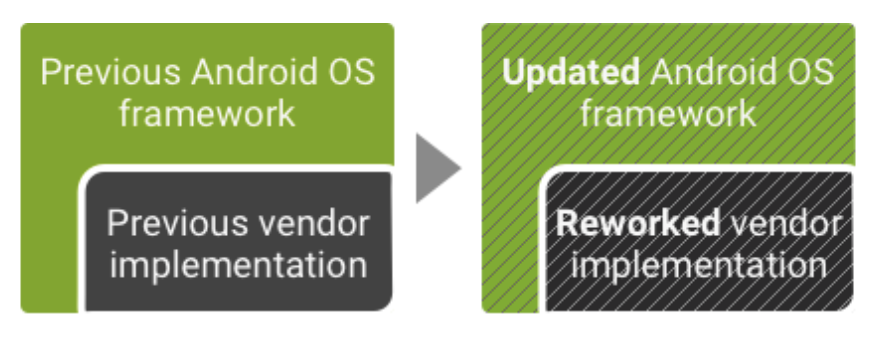
\includegraphics[width=0.5\textwidth]{treble1}
    \label{fig:LABEL}
\end{figure}

In Android 8.0+ (with Project Treble):
% Quick centered image
\begin{figure}[H]
    \centering
    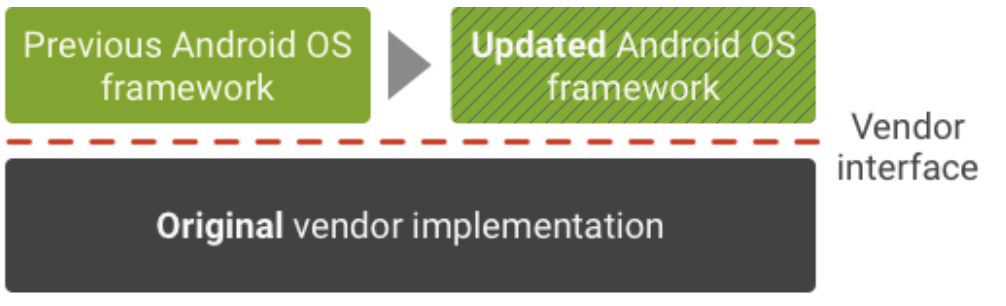
\includegraphics[width=0.5\textwidth]{treble2}
    \label{fig:LABEL}
\end{figure}

\section*{Most Devices (Still) Don't Get Security Patches}

Even with all this progress, many devices don't receive security updates

Most devices get support for only $\sim$3 years after launch (!= after you buy)

Some vendors (such as Google themselves) \textit{\textbf{slowly}} extend support: Pixel 8 and 8 Pro will get updates for at least 7 years. 

\section*{The Role of Security Researchers}

Identify malware
\begin{itemize}
	\item Once a new malware is found, it's added to blacklists
	\item Any app "similar" to the malware will be flagged and removed
\end{itemize}

Security vulnerabilities
\begin{itemize}
	\item Once they are found, they are reported to Google
	\item Monetary rewards for security bugs: "Bug Bounties"
\end{itemize}

Remember: attackers will also target anything not included in the bug bounties!

\textbf{Attacker Goals vs. Security Researchers}

Security researchers want to
\begin{itemize}
	\item Identify malware (add to disallow-lists, flag apps "similar enough" to listed malware apps) 
	\itme Report security vulnerabilities for bug bounties
\end{itemize}

Attackers want to
\begin{itemize}
	\item In general: run code on your device and do XYZ
\end{itemize}

Two main important topics:
\begin{itemize}
	\item Malware analysis, detection, containment
	\item Vulnerability analysis, detection, prevention, patching
\end{itemize}

\newpage
\begin{center}
  {\LARGE \textbf{Android Apps}}
\end{center}
\vspace{0.5cm}

\section*{Android apps in a Nutshell}

Apps are written in Java, C/C++, Kotlin, Rust, ...

Android apps "live" in the Android context
\begin{itemize}
	\item Android framework exposes a gigantic number of APIs
	\item APIs somewhat equivalent to "library functions"
\end{itemize}

APIs are useful for
\begin{itemize}
	\item Apps to interact with the "external world" (via
	\item The Android framework to interact with the Android app, e..g., where does the execution start?
	\item To extend Java SDK APIs: Many APIs from the Java world are part of the Android APIs 
\end{itemize}

\textbf{The size of documentation} for Android Framework APIs is \textbf{huge}!

Example of APIs: access to GPS/location info
\begin{lstlisting}[language=Java]
LocationListener list = new MyLocationListener();
list.requestLocationUpdates(LocationManager.GPS_PROVIDER, 5000,
	10, locationListener);

class MyLocationListener implements LocationListener {
	@Override
	public void onLocationChanged(Location loc) {
		Toast.makeText("Location" + loc.getLatitude() +
		", " + loc.getLongitude());
	}
}
\end{lstlisting}

\section*{Package Name}

Each app has a package name, e.g., "com.facebook.katana"

The package name acts as a "unique" identifier across the system

Constraints: package name needs to be *unique* 
\begin{itemize}
	\item across apps installed on a specific Android device
	\item across the \underline{Google Play Store}
\end{itemize}

\section*{Basics on Android apps}

There's no "main" function (like in C programs)

The user interacts via the Graphical UI
\begin{itemize}
	\item Many types of UI Widgets: \underline{EditText}, \underline{Buttons}, ...
	\item No command line interface
\end{itemize}

Many APIs are "event-driven"
\begin{itemize}
	\item You register a "listener" X
	\item X's callback is invoked later on
\end{itemize}

Apps are built as a combination of "components"


\section*{The Four Component Types}
\begin{itemize}
	\item Activity: entry point for interacting with the user. It represents a single screen with a user interface. You can have many: each of them defines a UI. Also, you can define which one is the "main" one. If app allows it, an external app can start these activates at will.
	\item Service: meant to perform an action in the background for some period of time, regardless of what the user is doing in foreground (the user could be witching between activities) e.g., Spotify
	\item Broadcast Receiver: meant to respond system-wide events. They have a well-defined entry point as well. The system can deliver these events even to apps that are currently not running. Examples: battery charging, SMS is received
	\item Content Provider: manage a shared set of app data. High-level API to access data so that other apps and services can query / interact with. Most often based on SQLite database (file-based). Example: calendar events, contacts list, settings
\end{itemize}

\begin{tcolorbox}[
  colback=orange!15,     % background color
  colframe=black!50,    % border color
  boxrule=1pt,       % border thickness
  arc=3mm,             % rounded corners
  left=4mm, right=4mm, top=2mm, bottom=2mm % padding
]
Each component type has its own life cycle
\end{tcolorbox}

\section*{Communication Between Components: Intents}

How can these components talk to each other?

Android-defined objects that encode an "Intent" (a fancy IPC message)

Examples: 
\begin{itemize}
	\item "Sharing content to an app", done via Intents
	\item "Choosing a file", send an Intent to FilePicker Activity
	\item "Open a webpage", send an Intent to the default Browser Acitivty
	\item "Take a picture", send an Intent to the Camera Activity
\end{itemize}

\section*{The Manifest File}

The most important file of an Android app

It specifies all key information needed by the framework to run the app:

\begin{itemize}
	\item Package name
	\item Components app consists of
	\item Intent filters
	\item Main Activity $->$ main() entrypoint
	\item Permissions
\end{itemize}

\section*{Android Studio}

Central/recommended IDE for Android app development

Common IDE features like
\begin{itemize}
	\item Syntax highlighting
	\item Go to Definition/Usage
	\item Tooling for compilation, packaging, deployment
	\item Tons of plugins: vim bindings!
\end{itemize}

Android-specific features like
\begin{itemize}
	\item Android Virtual Device (AVD) manager
	\item And much, much more...
\end{itemize}

Some people hate it: too slow, crashes, quirks, etc...

You can \textbf{compile it from the command line}! So you don't need Android Studio. 

% Quick centered image
\begin{figure}[H]
    \centering
    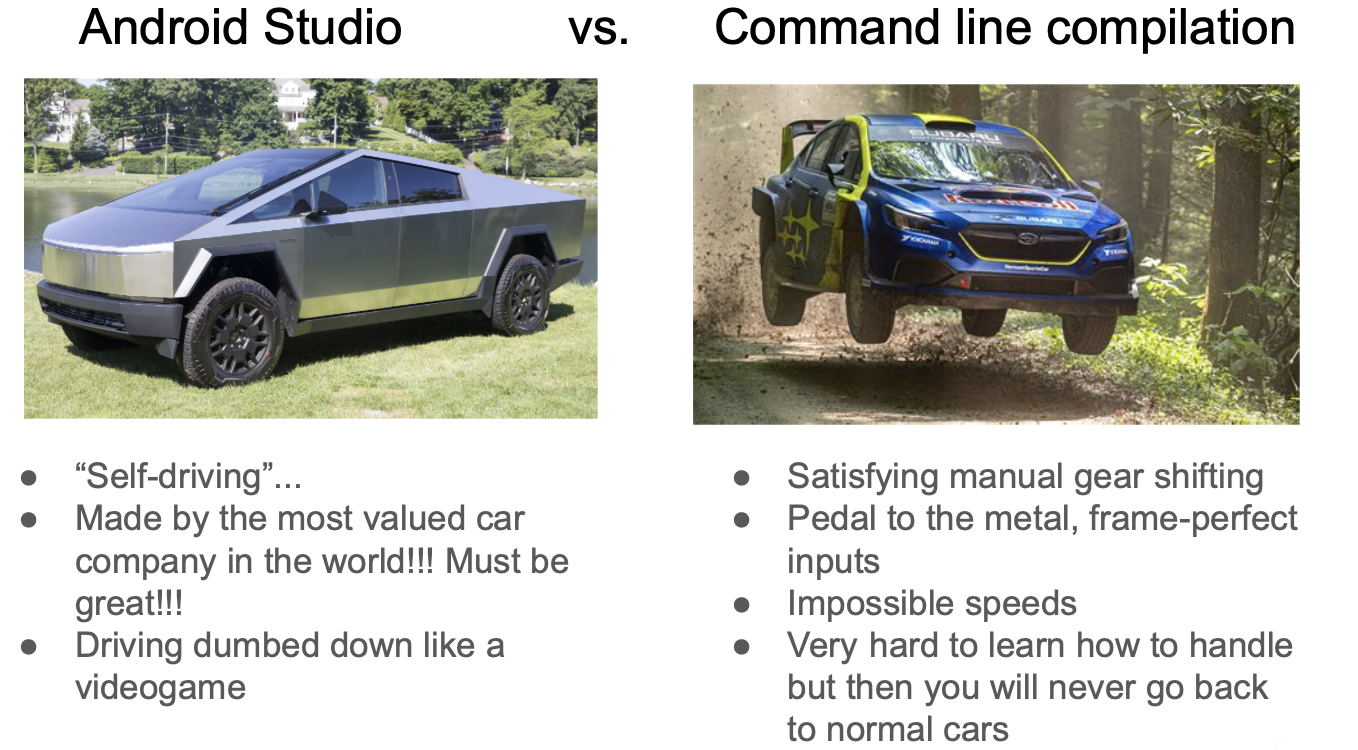
\includegraphics[width=0.8\textwidth]{compile}
    \label{fig:LABEL}
\end{figure}

\vspace{0.5cm}

\begin{center}
  {\LARGE \textbf{App Security}}
\end{center}
\vspace{0.5cm}

\section*{From the Eyes of an app}

Android is based on Linux. Each app has its own Linux user ID
\begin{tcolorbox}[
  colback=orange!15,     % background color
  colframe=black!50,    % border color
  boxrule=1pt,       % border thickness
  arc=3mm,             % rounded corners
  left=4mm, right=4mm, top=2mm, bottom=2mm % padding
]
There are ways to setup apps so that they share the user ID.
\end{tcolorbox}

Each app lives in its own security \textit{sandbox}
\begin{itemize}
	\item Standard Linux process isolation
	\item Restricted file system permissions
\end{itemize}

For \textbf{App installation}, the Android framework creates a new Linux user with a new user ID*

Each app is given a private direction
\begin{itemize}
	\item Also called "Internal Storage"
	\item No other app can access it
	\begin{tcolorbox}[
	  colback=orange!15,     % background color
	  colframe=black!50,    % border color
	  boxrule=1pt,       % border thickness
	  arc=3mm,             % rounded corners
	  left=4mm, right=4mm, top=2mm, bottom=2mm % padding
	]
	There are ways to setup app so that they share the user ID
	\end{tcolorbox}
\end{itemize}

\section*{Android Framework Architecture}

% Quick centered image
\begin{figure}[H]
    \centering
    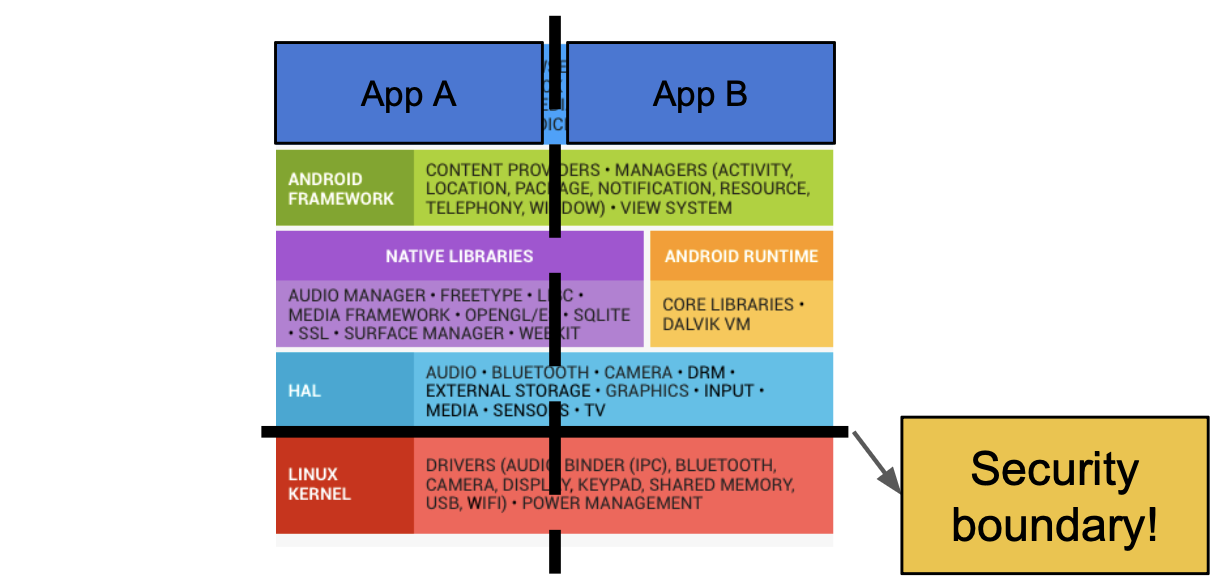
\includegraphics[width=1\textwidth]{android-framework-architecture}
    \label{fig:LABEL}
\end{figure}

\textbf{Be aware:} Malware is often written in native code without using any of Android Framework available tools! 

\textbf{syscalls} (Digression)

Traditional OSes (like Windows, Linux, Android) have two worlds: User-space vs. Kernel-space. Kernel-space commands are called \textbf{syscall}

\begin{itemize}
	\item User-space: where user processes and apps live: They can't do much by themselves (the JVM is also part of the user-space)
	\item Kernel-space is where the actual OS lives: The OS is the God of your machine and information
\end{itemize}

Some apps are different from the others: they are called \textbf{Managers}: \textit{They run as "privileged" users/apps!}. Examples: LocationManager, TelephonyManager, etc...

\section*{Example: getLastLocation()}

App invokes Android API:
\begin{itemize}
	\item \verb|LocationManager.getLastLocation()|
	\item We are still within the app's sandbox!
\end{itemize}

Actual implementation of the privileged API:
\begin{itemize}
	\item \verb|LocationManagerService.getLastLocation()|
	\item We are in a "privileged" service
\end{itemize}

How do we go from one side to the other one?

\section*{Crossing the Bridge}

Binder: one of the main Android's "extensions" over Linux

It allows for
\begin{itemize}
	\item Remote Procedure call (RCP)
	\item Inter-Process Communication (IPC)
\end{itemize}

Different from Intents:
\begin{itemize}
	\item Faster, lower level
	\item Allows for bidirectional client-server communication
\end{itemize}

\textbf{There are many "Managers" on Android phones}: Activity, Package, Telephony, Resource, Location, Notification, etc...

\section*{Android Permission System}

Android framework defines a long list of permissions

Each of these "protects" security-sensitive capabilities:
\begin{itemize}
	\item The ability to "do" something sensitive, e.g., open Internet connection, send SMS
	\item The ability to "access" sensitive information, e.g., location, user contacts, ...
\end{itemize}

\textbf{Examples of Permissions:} \verb|INTERNET|, \verb|SET_WALLPAPER|, \verb|BLUETOOTH|, ...

\newpage
\begin{center}
  {\LARGE \textbf{Reversing Android Apps}}
\end{center}
\vspace{0.5cm}

The compilation process

% Quick centered image
\begin{figure}[H]
    \centering
    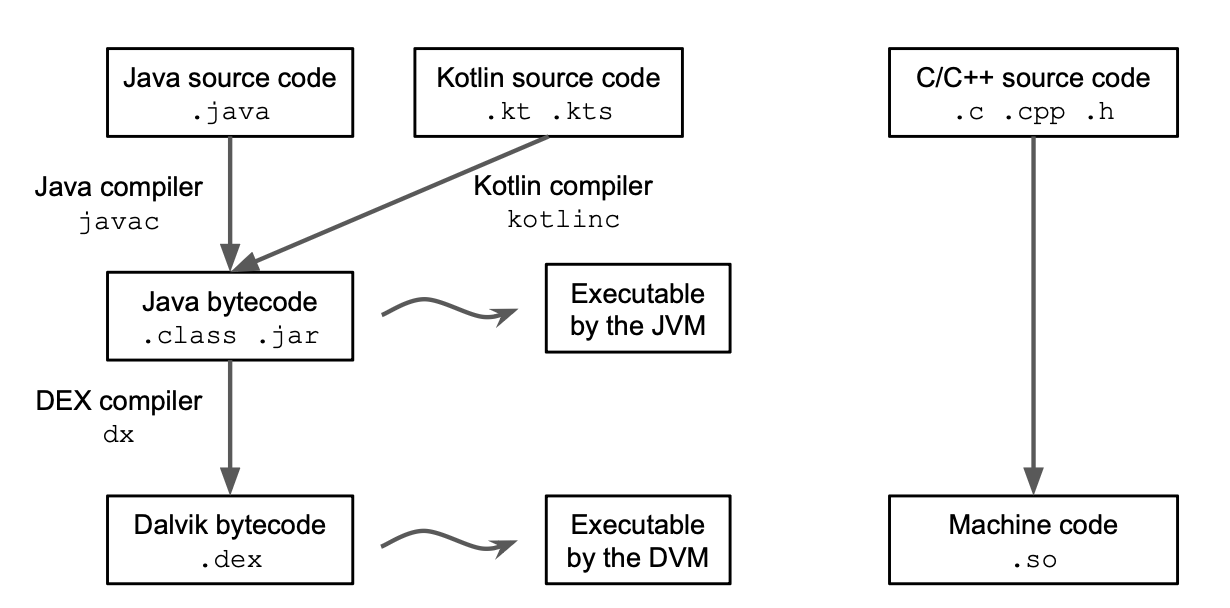
\includegraphics[width=0.7\textwidth]{compile-process}
    \label{fig:LABEL}
\end{figure}

\section*{Android Application Package (APK)}

An APK is a zip file (with a magic format). Its content is:
\begin{itemize}
	\item \verb|AndroidManifest.xml| (compressed)
	\item \verb|classes.dex| (raw Dalvik bytecode)
	\item \verb|resources.arsc| (compressed)
	\item \verb|rest/*.xml| (compressed)
\end{itemize}

The big picture

% Quick centered image
\begin{figure}[H]
    \centering
    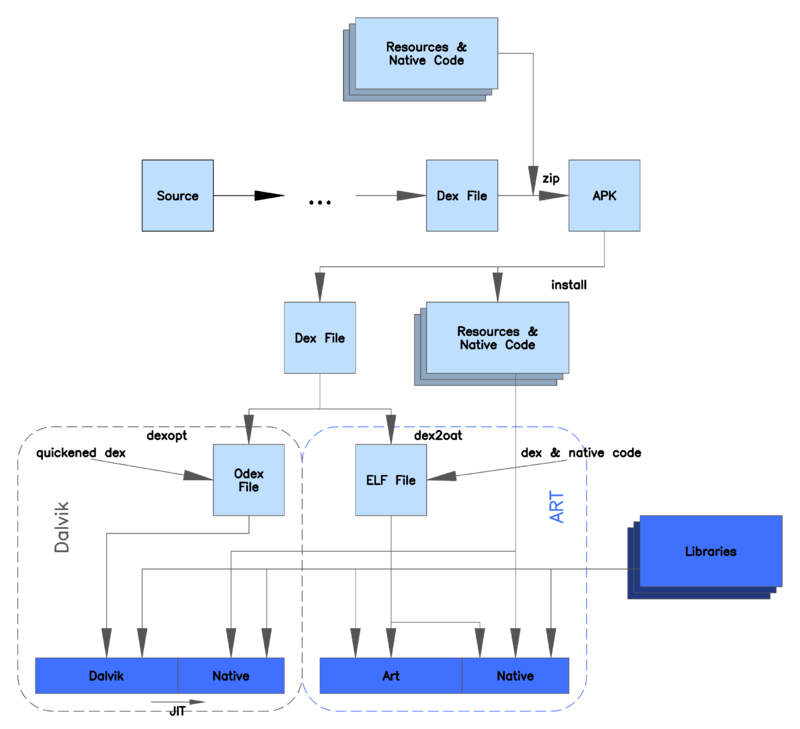
\includegraphics[width=0.5\textwidth]{big-picture}
    \label{fig:LABEL}
\end{figure}

\section*{How to Decompile}

All-in-one tools
\begin{itemize}
	\item Jadx (top tool, check out first)
	\item JEB (commercial, VERY expensive)
	\item BytecodeViewer (pretty good one) 
	\item New: Ghidra, open source tool developed by NSA
\end{itemize}

Using a Java decompiler (java bytecode $\Rightarrow$ Java)
\begin{itemize}
	\item Dalvik bytecode $\Rightarrow$ Java bytecode, e.g., Dex2jar
	\item Java bytecode $\Rightarrow$ Java source code, e.g., Jd-GUI
\end{itemize}

\textbf{How people find bugs:} \textit{decompiling} apps and \textit{analyzing} them
\vspace{0.5cm}

\begin{center}
  {\LARGE \textbf{Android Security Mitigations}}
\end{center}
\vspace{0.5cm}

\section*{Android Implements Defense in Depth}

Multiple layers of security controls are placed throughout the system. It prevents single vulnerabilities from leading to compromise of the OS or other apps

\begin{itemize}
	\item \textbf{Application Sandbox}: Apps are isolated from each other by being assigned to different users. The sandbox is in the kernel: native code can't bypass it. To bypass the sandbox, an attacker would need to compromise Linux. \textbf{Chain of 2 bugs!}
	\item \textbf{SELinux (Mandatory Access Control)}: Security-Enhanced Linux: a Linux kernel security model
		\begin{itemize}
			\item Useful to defined MAC security polices
			\item Example: allow/prevent execution of syscall X
			\item "Deny by default" policy 
		\end{itemize}
	All processes labeled with the same domain are treated equal. Currently there are 60+ domains in Android
	\item \textbf{ARM MTE (Memory Tagging Extension}: Add a "tag" in the unused, upper bits of a pointer. The tag defines which memory area the pointer is allowed to target. Every load/store is checked, raise exception if pointer goes out of bounds. Mitigates against: buffer overflows, use-after-free. Available since Android 12 on ARMv9 compatible CPUs. 
	\item \textbf{Scudo (Hardened Heap Memory Allocator}: Improved version of malloc with some additional features.
		\begin{itemize}
			\item Randomized allocations
			\item Guard pages to prevent some heap overflows
			\item More information stored in chunk headers to detect some types of double frees
		\end{itemize}
		However, this mitigation has been bypassed multiple times, it only slightly complicates exploitation. Enabled since Android 11.
	\item etc... Nowadays, to obtain \textbf{complete control} over a mobile phone, you need to chain \textbf{5-6 bugs}. 
\end{itemize}

\vspace{0.5cm}

\begin{center}
  {\LARGE \textbf{Android vs. iOS}}
\end{center}
\vspace{0.5cm}

\begin{minipage}{0.45\textwidth}
\textbf{Android} \\
\begin{itemize}
	\item $\sim$ Open source \\
	\item Customizable \\ 
	\item Targeting everyone \\
\end{itemize}
Strong candidate but...

\end{minipage}
\hfill
\begin{minipage}{0.45\textwidth}
\textbf{iOS} \\
\begin{itemize}
	\item Corporate \\
	\item Closed, conservative \\
	\item Targeting the rich \\
\end{itemize}
Somehow still wins...
\end{minipage}

In \textbf{Switzerland}, iOS is leading the market as of \textbf{India}, Android is dominant (95\%)

\section*{Apple's Strategy}

Apple's iOS ecosystem is \textbf{\textit{extremely closed}}
\begin{itemize}
	\item iOS is closed source
	\item iOS and iOS apps can only run on Apple devices
	\item \textit{You can install apps only from the Apple Store} (changing due to EU legislations)
	\item Apps need to be signed from the developer \textit{and} Apple
	\item Not easy to "jailbreak" iOS devices anymore
\end{itemize}

How come they are still around?
\begin{itemize}
	\item They were the first $\Rightarrow$ significant chunk of market share
	\item They make great products, and people know about it
\end{itemize}

\section*{Google's Strategy}

Android Inc. (purchased by Google in '05) started developing Android '03

Google needed to catch up: "Open Handset Alliance" (84 companies)

Ecosystem is much \textit{\textbf{more}} open in principle
\begin{itemize}
	\item Android / AOSP is open source
	\item Android can run on many different devices, even non-Google ones
	\item Easy to inspect Android apps / reverse them / modify them
	\item Easy to install apps you develop ("side loading")
	\item Developers can do many more things
	\item Quite easy to "jailbreak" Android devices
\end{itemize}

\section*{Android is becoming closed like iOS}

Ecosystem \textit{was} more open
\begin{itemize}
	\item AOSP is open source but many critical components are not (e.g., DRM libraries or vendor specific components)
	\item Many obfuscated apps (e.g., Whatsapp)
	\item Jailbreaking devices has become hard (as vendors force you to jump through weird obstacles, e.g., Xiaomi requires creating an account)
	\item Many apps refuse to work with a "customized" device (e.g., Google services, bank apps, etc) 
\end{itemize}

\section*{Open vs closed source}

\begin{tcolorbox}[
  colback=orange!15,     % background color
  colframe=black!50,    % border color
  boxrule=1pt,       % border thickness
  arc=3mm,             % rounded corners
  left=4mm, right=4mm, top=2mm, bottom=2mm % padding
]
\textbf{Kerckhoff's principle}: a cryptosystem should be secure, even if everything about the system, except the key, is public knowledge! (Cryptographic point of view)
\end{tcolorbox}

% Quick centered image
\begin{figure}[H]
    \centering
    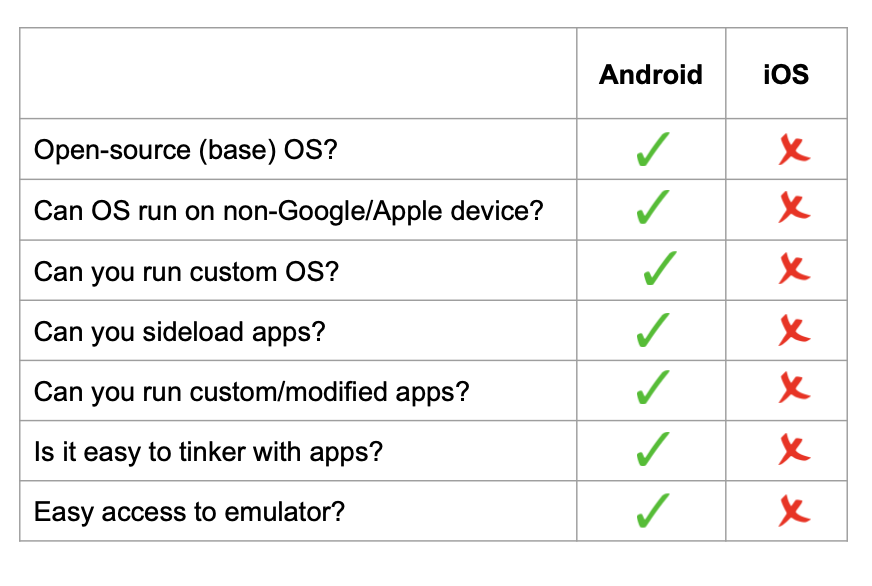
\includegraphics[width=0.6\textwidth]{open-closed}
    \label{fig:LABEL}
\end{figure}

\vspace{0.5cm}

\begin{center}
  {\LARGE \textbf{The mobile exploit market}}
\end{center}
\vspace{0.5cm}

\textbf{Mobile exploit payouts are exploding!}

Full remote chain on Samsung S24: only 50,000\$ (2024). Which is really low as bounty.

\textbf{Cellebrite} iPhone support (to dump file system) 

They have compatible versions with latests versions and iPhones which require AFU = After First Unlock (i.e., is the encryption key loaded in RAM?) iPhone support (to dump file system) 

They have compatible versions with latests versions and iPhones which require AFU = After First Unlock (i.e., is the encryption key loaded in RAM?) 

\textbf{If you are in trouble, turn off your phone!}

\section*{GrapheneOS}

Custom Android distro, ultra-hardened and privacy focused

\begin{itemize}
	\item Extremely reduced attack surface (e.g., way less USB features)
	\item Actually hardened malloc
	\item Prevent VPN leaks
	\item Hardened PDF viewer
	\item No Google apps/play services
	\item No zygote (users ASLR/canaries)
\end{itemize}

\section*{iOS Lockdown mode}

When Lockdown Mode is enabled, some apps and features will function differently. It protects your device in many ways...

\section*{What is the US president using?}
\begin{itemize}
	\item Hyypervisor-based Android distro
	\item Almost no details are public
	\item Price not reported (i.e., very expensive)
\end{itemize}

\section*{Summary}

Mobile security is different from OS/desktop

Android is much more open and customizable than iOS. Android can be made very safe, or very unsafe. iOS restricts users to a pretty good baseline, but it's not customizable. 

Mobile ecosystems rely on many layers of security, on system, during boot, and across different trust levels (e.g., trust zone)

Android fragmentation remains a key challenge 

Apps are checked in the central market and build on the ecosystem

App security may be an issue: outdated libraries and fragmentation

\end{document}
